\documentclass[10pt]{article} % Font size - 10pt, 11pt or 12pt

\usepackage[hmargin=1.25cm, vmargin=1.5cm]{geometry} % Document margins

\usepackage[usenames,dvipsnames]{xcolor} % Allows the definition of hex colors

% Fonts and tweaks for XeLaTeX
\usepackage{fontspec,xltxtra,xunicode}
\defaultfontfeatures{Mapping=tex-text}
%\setmonofont[Scale=MatchLowercase]{Andale Mono}

% Colors for links, text and headings
\usepackage{hyperref}
\definecolor{linkcolor}{HTML}{506266} % Blue-gray color for links
\definecolor{shade}{HTML}{F5DD9D} % Peach color for the contact information box
\definecolor{text1}{HTML}{2b2b2b} % Main document font color, off-black
\definecolor{headings}{HTML}{701112} % Dark red color for headings
% Other color palettes: shade=B9D7D9 and linkcolor=A40000; shade=D4D7FE and linkcolor=FF0080

\hypersetup{colorlinks,breaklinks, urlcolor=linkcolor, linkcolor=linkcolor} % Set up links and colors

\usepackage{titlesec}
\setcounter{secnumdepth}{4}

\titleformat{\paragraph}
{\normalfont\normalsize\bfseries}{\theparagraph}{1em}{}
\titlespacing*{\paragraph}
{0pt}{3.25ex plus 1ex minus .2ex}{1.5ex plus .2ex}

\usepackage{fancyhdr}
\usepackage{amssymb}
\usepackage{amsmath}
\pagestyle{fancy}
\fancyhf{}

\renewcommand{\headrulewidth}{0pt} % Get rid of the default rule in the header

\bibliographystyle{plain}

\begin{document}

\tableofcontents
\newpage

\section{Chapter: Introduction}
\subsection{What is dynein?}
\subsubsection{Basics}

Dynein is a cellular structure which converts chemical energy to mechanical energy. It does so by reacting with adenosine triphosphate (ATP) to take steps along long cellular tracks known as microtubules. Dynein's mechanical energy is used to transport molecules around the cell, pull chromosomes during division, move cellular propellers known as cilia
and various other functions \cite{cianfroccoreview}.\\

A depictions of dynein is shown in Figure (\ref{dynein-artist-rendition}).\\

\begin{figure}[h]
  \centering
  \includegraphics[width=.65\textwidth,keepaspectratio]{../figures/dynein-artist-rendition-2.jpg}
  \caption{Artist rendition of the dynein motor. Modified. Source: Lander Lab, The Scripps Research Institute.}
  \label{dynein-artist-rendition}
\end{figure}

Dynein is believed to move by using the energy of ATP to cycle through a ring of states, each with different spatial relations to the microtubule. By cycling forward through this ring, the molecule can end up in the same state it began, but moved forward a small amount. This ring of states is known as the mechanochemical cycle \cite{cianfroccoreview}.\\

The goal of this project is to create a mathematical model of the mechanochemical cycle and verify that it can reproduce experimental dynein stepping data.\\

\subsection{Biology review}

\textit{This section will describe everything people need to know about dynein to understand the project: what proteins are, what dynein does, the things it uses to do it, and why it is necessary. Show a crystal structure as well as artist's rendition.}

\subsubsection{Why do cells need motor transport?}
Cells are structures with high organization in time and space. 
Cells are organized, heretogenous structures which respond quickly to their environments. This means that cells require a mechanism for rapidly moving cargo, and moving cargo to precise locations within the cell. This can be a challenge, since cells are fairly large compared to the proteins which compose them \textbf{is it also a challenge because its hard to get precise positions within a cell?}. A human fibroblast cell has a volume of roughly 2000 $\mu m^3$\cite{fibroblastvolume}, corresponding to roughly $8 \mu m$ in diameter. In comparison, human hemoglobin has a diameter of roughly $5 nm$ (PDB id 5ME2) \textbf{((is this the best way to cite this?))}, a $10^3$ factor difference in size.\\

Diffusion, or random motion of molecules due to collisions with solvent (i.e. Brownian motion), is one possible means cells could use to transport cargo. Diffusion has two problems: it is slow and nondirected. The expected distance covered for one-dimensional Brownian motion after time t was found by Einstein to be \textbf{cite here}:

\begin{equation}
  \label{diffusion-equation}
  <x> = \sqrt{2Dt}
\end{equation}

where D is the diffusion constant (flesh this out). The $\sqrt{t}$ scaling of diffusion contrasts with the linear scaling of motor transport. 

This ties in a lot to the previous section. I originally thought of putting the <x> vs T diffusion/
motor plot in the introduction, but maybe it would be better here. Not sure.\\

\subsubsection{What role does it play in the cell?}
This'll require more reading...dynein transports cargo, such as proteins, vesicles, and other cellular structures. How does binding to structures work, is it random Brownian? Do dyneins bind to the MT then cargo, or vice versa? What does dynein actually bind to, since it has a single binding domain that
can't recognize everything. Does it have different binding partners which bind to specific things?\\

Other roles than transport: moving around microtubules to help with chromosome segregation, what else?

\subsubsection{How does it behave?}
Talk about its stepping behavior using Weihong's figures (as well as the new paper David found?)\\

Also possibly talk about the other things Dynein has been found to do, such as hydrolyse ATP and
move its subdomains around. This may be better in a different section than the introduction though,
since its a lot of biochemistry for the second section in an intro? maybe not, it has to go somewhere.

\subsubsection{Why is dynein special and interesting?}
Compare the processive motion of dynein to kinesin in \textbf{a.)} directionality, \textbf{b.)}
stepping pattern and \textbf{c.)} size (like how it can step over roadblocks kinesin cannot).\\

Talk about why a random stepping motor is interesting compared to a orderly-stepping motor: what
is different about dynein's structure that makes it step differently? Compare the crystal structures
and ask lots of questions. Build interest in the motors here.\\

\subsection{How does dynein walk?}
Show the \textit{Cianfrocco} annual review figure on the mechanochemical cycle of dynein. Talk about
how each step works in some detail, according to the theory. Find out what other papers say about
this cycle, and whether there is disagreement about how the cycle works.


\subsubsection{Experimental results on dynein’s step}
Weihong's figures go here.\\
\subsubsection{Experimental features of dynein (ATPase, multi-state…)}
Some history of studies which have determined what dynein has in it.\\

\subsubsection{Powerstroke Theory}
Talk about the history of this idea, why it is supported and why it is not supported.\\
\paragraph{The theory}
Describe the theory.
\paragraph{b Evidence of theory}
Evidence supporting the powerstroke.

\subsubsection{c What is still needed to support theory}
Where our simulation fits in. Why we need this kind of information.
\subsubsection{Other theories?}
	\subsection{Past Simulations}
		\subsubsection{Why simulations are necessary}
		\subsubsection{Sarlah Winch Model}
		\subsubsection{-x Other models}
	\subsection{Brownian motion}
                \subsubsection{Introduction/derivation}
                \subsubsection{Justification}
\section{Chapter: Methods}
\subsection{Simulation}
Talk about why simulation is the only way to verify the mechanochemical cycle, since experiments
aren't high resolution enough to make good videos of the walk, and even if they were, in some sense
knowing that dynein behaves identically to a simple mathematical model is more informative than
a video, since there is lots of information in a video and really precise info in a simulation.\\

\textbf{Not sure where this goes:} The 'goal' of our experiment, at a very high level, is to
understand how dynein works. We can know this if we can come up with the minimum set of characteristics a physical system needs to act like dynein. This information is the same thing as knowing
``how dynein walks.'' We don't need to know all the complex dynamics of every single amino acid in
dynein, we only need to know our rough model.\\

\subsection{Our model}
Talk about what the important parts of the mechanochemical cycle from the introduction are, and how
we take those and model them.\\
\subsubsection{Rigid point model}
Talk about two things: reducing bulky circular domains to points (is this the same as unified atom
model?) with a certain drag constant based on radius, and acting like the domains are rigid in
distance from each other. Talk about why this is valid (is it? it's an assumption, David may know
more).
\subsubsection{Harmonic energies}
How we're modeling the complicated folding and adjusting of a massive protein as a harmonic
oscillator. Why this is valid. Also other approaches...what else could we have modelled it as?
\subsubsection{Two-state model}
The mechanochemical cycle has eight states. We choose two as representative because \textbf{a.)}
many of the states are identically conformationally or \textbf{b.)} the transitions happen so fast
the intermediate states don't matter. Talk about rate constants here.
\subsubsection{Limitations}
Talk about the things we \textit{don't} take into account...motor-motor interaction, 2d information,
other ATPase nucleotide state, saying certain mechanochemical steps occur ``fast,'' not taking into
account all mechanochemical cycle states, making the coiled coil domain rigid even though it may be
springy...

\subsection{Simulating our model}
Talk generally about what simulating stuff means.\\
\subsubsection{Motion equations}

\paragraph{a Onebound solution}
Discuss how our model is represented by the following figure (maybe get one with springs on the
hinges):\\

\begin{figure}
  \centering
  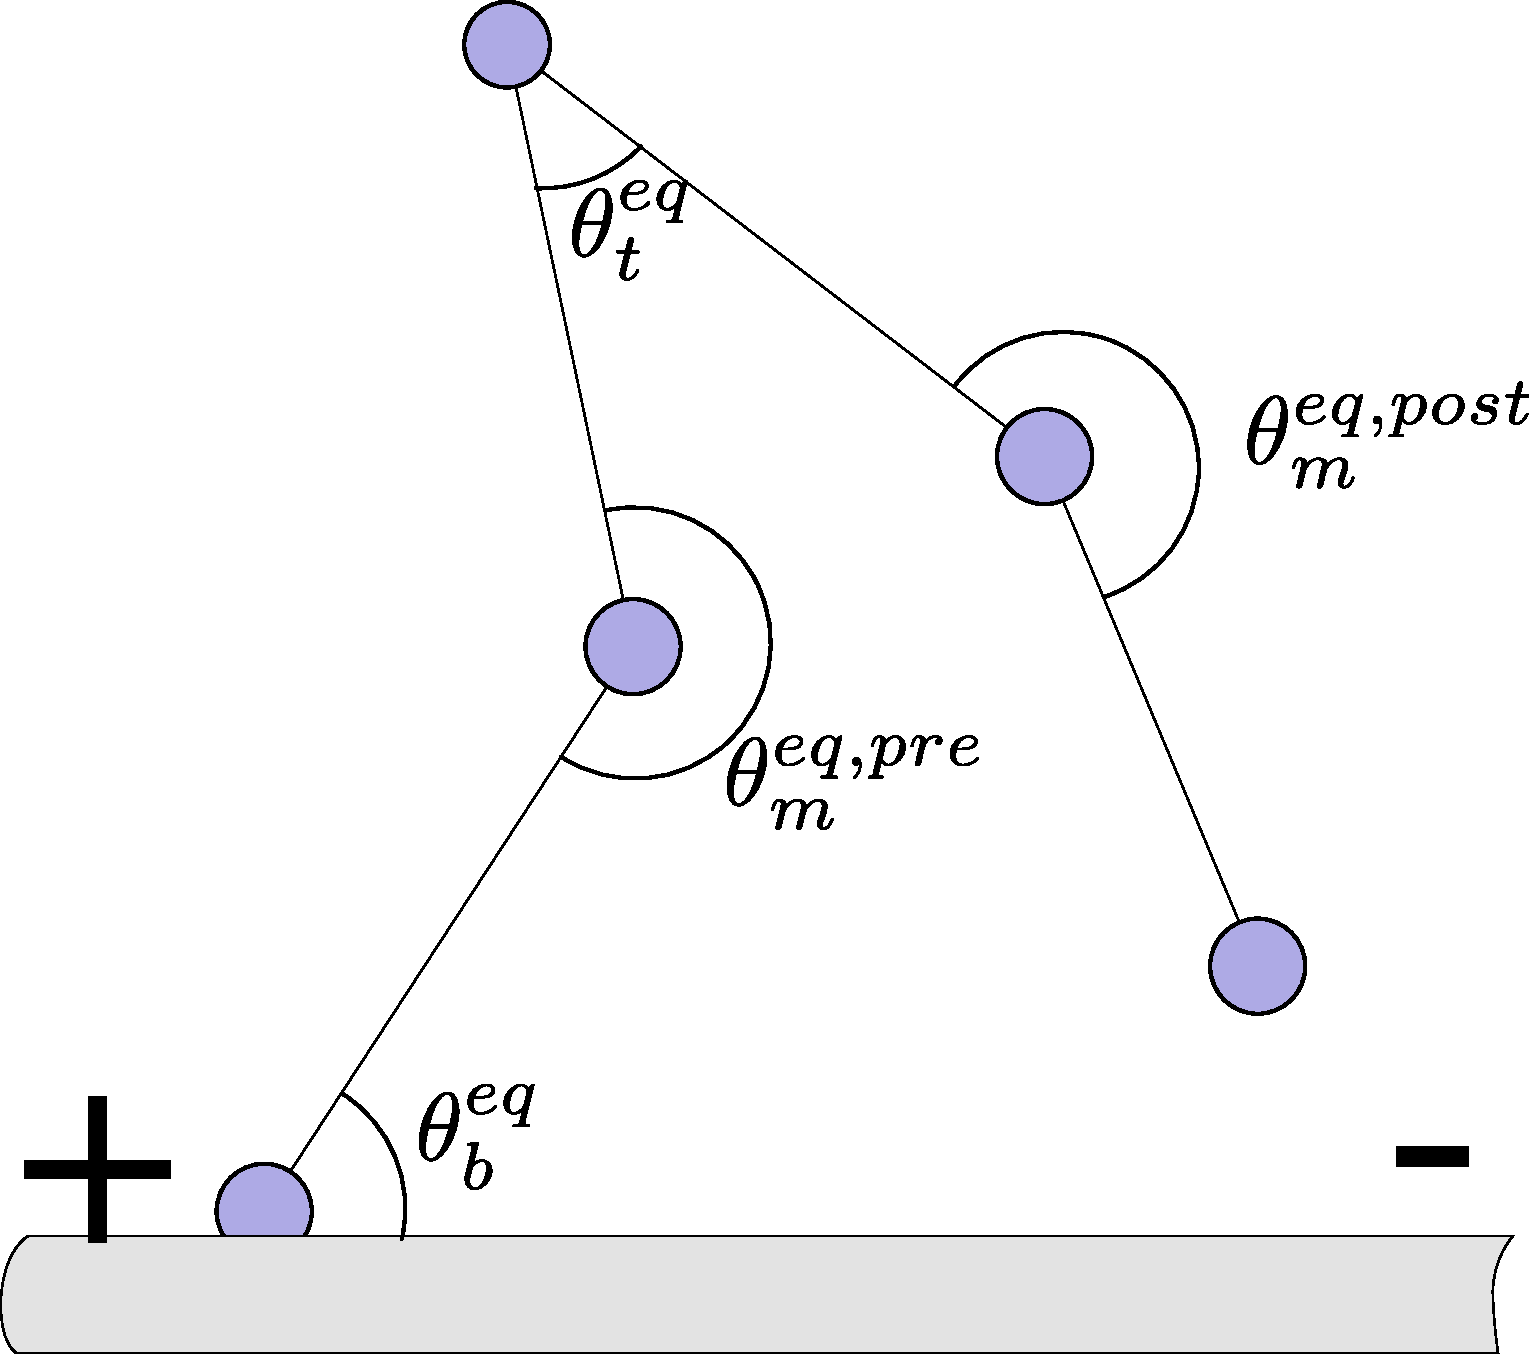
\includegraphics[width=.45\textwidth]{../figures/equilibrium-onebound}
  \caption{Definition of equilibrium angles.}
  \label{fig:eq_angles}
\end{figure}

Show the derivation process.\\

\paragraph{b Bothbound solution}
Show how bothbound is derived and different from onebound. Put the actual equations in the appendix,
or just leave them out 'cause they're ugly?\\

\subsubsection{Code}
Talk about using C++, Make, C, Python. Talk about the rough program flow, how we go from code to
data.\\

\paragraph{a Running, compiling, language choice?}
Details on why we chose C++.\\
\subsubsection{Time evolution}
How we do time evolution.
\paragraph{Euler’s method}
Show how Euler's method is arrived at, how its error scales, why we use it.

\paragraph{Vs other methods (Runge Kutta, etc)}
Talk about why our differential equation is most conducive to Euler's method. Euler's is more
efficient -- is there a way to show how our differential equation is smooth, not jagged?

\paragraph{Finding the right dt}
Figure on error rate vs. dt.

\paragraph{State transitions}
Talk about how we calculate transition rates based on differences in energies between states.
Then how we use transition rates to transition our model accurately.\\

\paragraph{Gibbs energy of transition}
Do some stuff with Gibb's here? Why our energies are Gibb's and not internal energy?\\

\subsection{Verifying our model}
Talk about why we think our model accurately represents the system we are trying to model, and
doesn't have bugs in it.\\

Talk about this figure:

\begin{figure}[h!]
  \centering
  \begin{minipage}[b]{0.49\textwidth}
    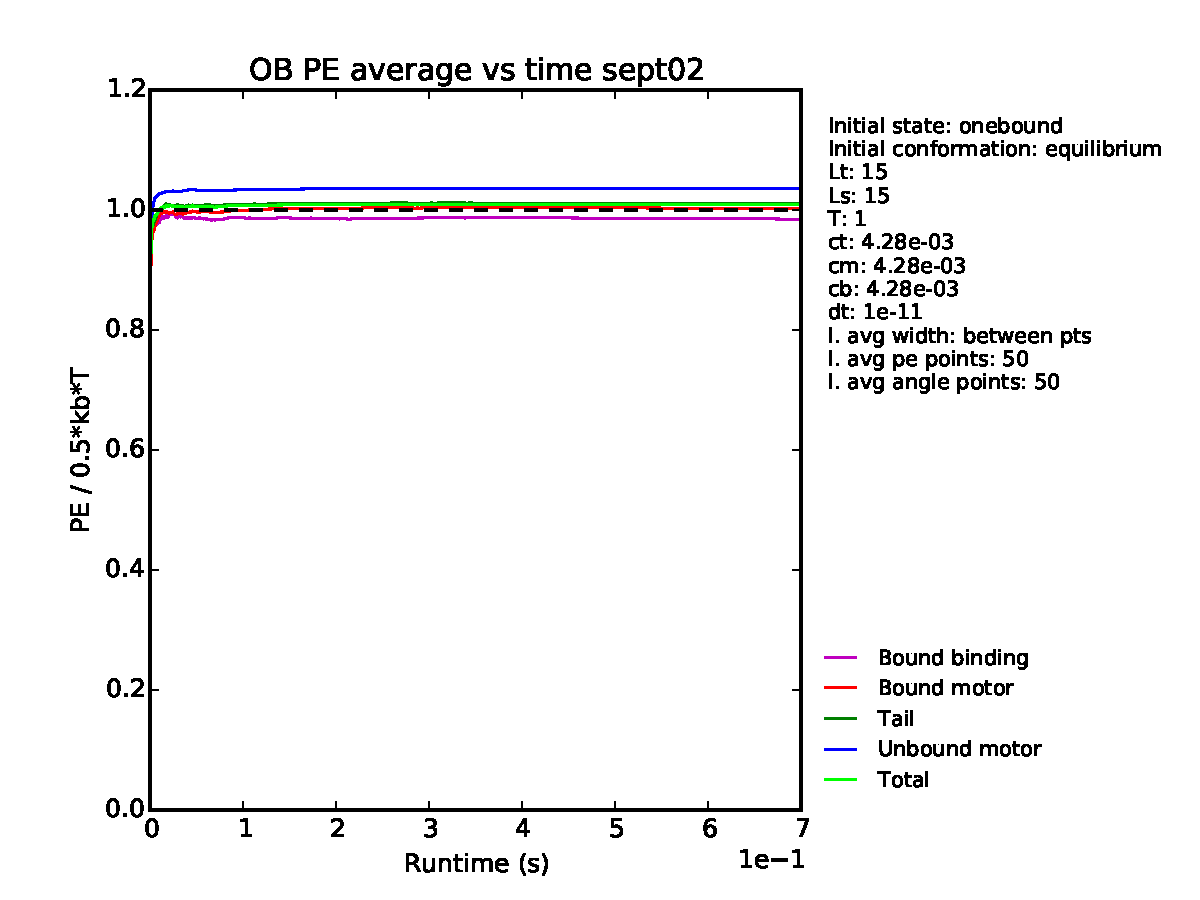
\includegraphics[width=\textwidth]{../figures/OB_Average_PE.pdf}
    \caption{Onebound PE vs time.}
  \end{minipage}
  \begin{minipage}[b]{0.49\textwidth}
    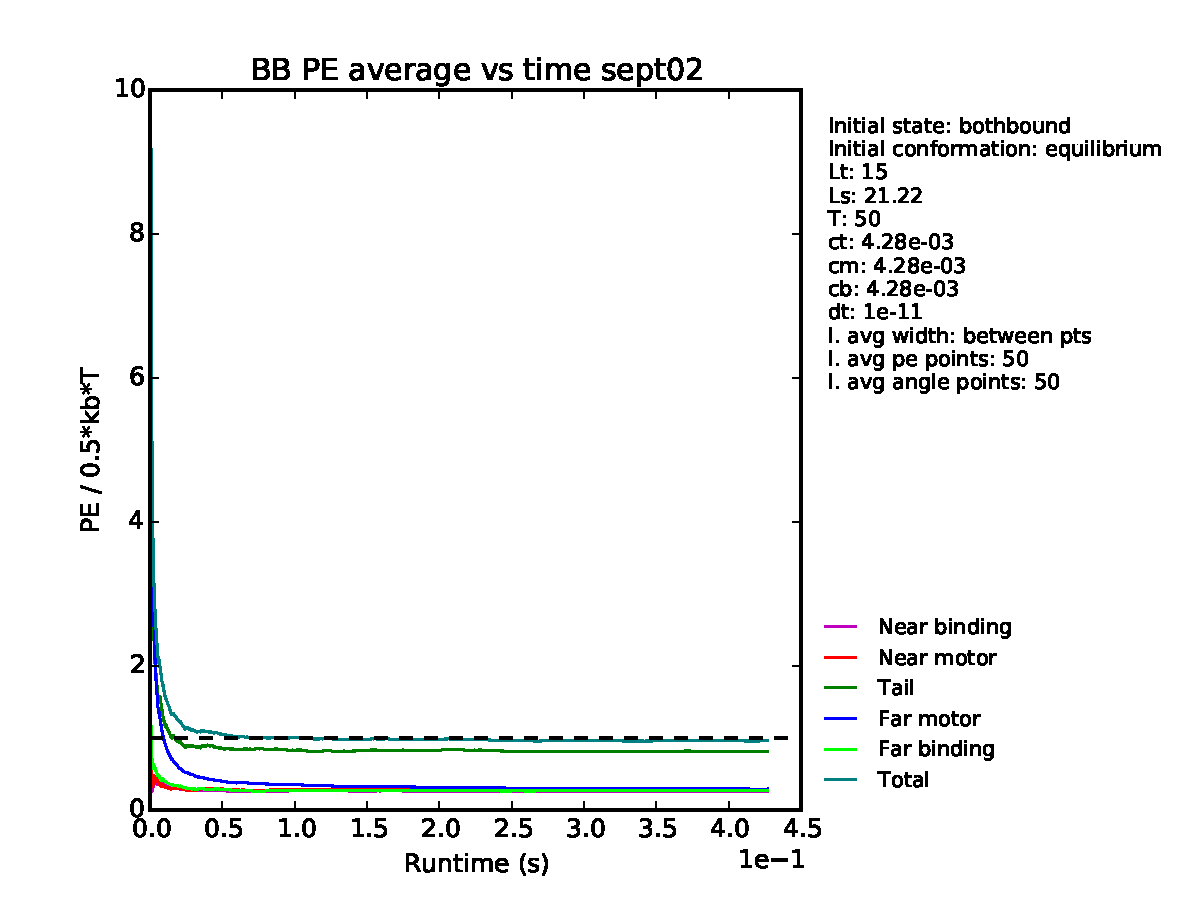
\includegraphics[width=\textwidth]{../figures/BB_Average_PE.pdf}
    \caption{Bothbound PE vs time.}
  \end{minipage}
  \label{fig:equipartition_agreement}
\end{figure}

and how it shows our model is physical, or at least, how obeying the equipartition theorem shows
how our domains both feel harmonic energies and can fully explore their spaces?\\

\subsection{Parameters}
The following table shows our guess parameters from various papers/crystal structures.\\
                        
                        \begin{center}
  \begin{tabular}{| l | l | l | l | l | l |}
    \hline
    & Winch (Sarlah) & Schmidt & Lin & PyMol 3VKH & PyMol 4RH7\\\hline
    $L_s$ & 12nm & & & 21.0nm & 22.1nm\\ \hline
    $L_t$ &  7nm & & & & 11.15nm\\ \hline
    $R_b$ &  & & & 1.57nm & 1.45nm\\ \hline
    $R_m$ &  7nm & & & 7.36nm & 6.3nm\\ \hline
    $R_t$ &  & & & & 2.16nm \\ \hline
    $\theta_{m}^{Pre}$ & 250$^{\circ}$ & & 171$^{\circ}$ & &\\ \hline
    $\theta_{m}^{Post}$ & 330$^{\circ}$ & & 137.5$^{\circ}$ & &\\ \hline
    $\theta_{b}$ & 56$^{\circ}$ & & 63.5$^{\circ}$ & &\\ \hline
    $\theta_{t}$ & 0$^{\circ}$ & & & &\\ \hline
    $k_{ub}$ & $180 s^{-1,a}$ & & & &\\ \hline
    $k_b$ & $5000 s^{-1,b}$ & & & &\\ \hline
  \end{tabular}
\end{center}
		\subsubsection{Lengths, angles, binding constants, etc…}
	\subsection{Tuning our model}
	\subsubsection{Searching for optimal parameters}
\section{Chapter: Results}
	\subsection{Histograms}
		\subsubsection{Step length histograms}
		\subsubsection{Step time histograms}
	\subsection{Other ways to represent data?}


\section{Chapter: Discussion}
\subsection{Why our model worked, didn’t work}
Fill this out over winter when you know more.\\
\subsection{Future work on this project}
If setbacks happen, this'll be a big section. Or, further simulations which could be done.

\subsubsection{Experiments to verify our model}
Talk about how FRET could be used to verify our model. We have domain distance info over long
timescales in our model - this is something we could compare to a FRET experiment exploring
the distance between domains in dynein.\\

Other biophysics experiments which could verify our model?\\

Calorimetry could get Gibb's energy of binding if you froze the motor in onebound using
vanadium? Maybe...\\
\subsection{Possible further projects}
\subsection{Difference between dynein and kinesin}
Our project un/successfully predicted how dynein behaved. How would we modify it to describe kinesin?
Is dynein's linker-motor connection less tense than kinesin's, leading to more random motion? This
would likely be lots of speculation, but it could be cool to look up some papers on kinesin motility
and get its crystal structure to do some comparisons.

\bibliography{thesis}

\end{document}
